\documentclass{myclass}
\usepackage{verbatim}
\usepackage{array}
\usepackage{listings}
\usepackage{fancyvrb}
\usepackage{enumitem}

\usepackage[utf8]{inputenc}
\usepackage[T1]{fontenc}
\usepackage{textcomp}
\usepackage{multicol}
\usepackage{mathtools}
\usepackage{amsmath}
\usepackage{wrapfig}
\usepackage{amssymb}
\usepackage{amsmath,amsfonts,amssymb,amsthm,epsfig,epstopdf,titling,url,array}
\usepackage{hyperref}
\usepackage{eso-pic}
\usepackage{pgf}
\usepackage{tikz}
\usepackage{graphicx}
\usepackage{tikz-cd}


% figure support
\usepackage{import}
\usepackage{xifthen}
\pdfminorversion=7
\usepackage{pdfpages}
\usepackage{transparent}
\usepackage{xcolor}

\setlength{\parindent}{0em}
\setlength{\parskip}{1em}

\newtheorem*{definition}{Definition}
\newtheorem*{theorem}{Theorem}
\newtheorem*{proposition}{Proposition}

\newcommand{\incfig}[1]{%
\center
\def\svgwidth{0.9\columnwidth}
\import{./figures/}{#1.pdf_tex}
}

\newcommand{\incsvg}[1]{%
\center
\def\svgwidth{0.9\columnwidth}
\import{./figures/}{#1.svg}
}

\newcommand{\incimg}[1]{%
\center
\includegraphics[width=0.9\columnwidth]{images/#1}
}
\pdfsuppresswarningpagegroup=1

\title{Notes on Coxeter Matroids}

\begin{document}
\maketitle
\tableofcontents
\newpage

\section{Matroids}
\begin{definition}[Matroid]
A base of a matroid M over a given a ground set $[n]$ is $\mathcal{B}(M)\subseteq \choose{[n], r}$, where $r$ is the rank of the matroid. The set  $\mathcal{B}$ must fulfill:
\begin{itemize}[topsep=-6pt, itemsep=0pt]
  \item $A, B \in \mathcal{B}, a\in A-B \Rightarrow \ \exists b\in B-A : (A-\{a\})\cup \{b\}\in \mathcal{B}$
\end{itemize}
\end{definition}

\section{Permutahedron}
\subsection{Regular permutahedron}
The permutahedron $\Pi_n$ is generated by the convex hull of the vertices $V = \{(\sigma(1), \ldots \sigma (n)) : \sigma \in S_n \}$

There is a (fancy) bijection between the flags of $[n]$ and the faces of permutahedron $\Pi_n$ as shown in the picture.

Flags could be interpreted as ordered partitions. One example of the three points of view as follows: $F = \{\{3\}, \{1, 2, 3, 4\}\} \iff 3|124 \iff$ "the face whose vertices have a $3$ in the first position and the other three are free permutations".

\begin{minipage}{\textwidth}
\incfig{PermutahedronBijectionFlags}
\end{minipage}

\subsection{Generalized permutahedra}

\begin{definition}[Hypersimplex] 
  $\Delta(n, k)=\{(x_1, \ldots, x_n): x_1 + \ldots+ x_n = k\}$
\end{definition}

The basis of $\Delta(n,k)$ (vertices of the polytope) is formed by vectors with $k$ ones and  $n-k$ zeroes.

\begin{definition}[Generalized Permutahedron] Convex polytope with all the edges parallel to $e_i-e_j$
\end{definition}

Permutahedron vertices came from a subset of the vertices of $\Delta(n, k)$

 \begin{definition}[Matroid polytope] Matroid generated by the permutahedron whose vertices are a subset of $\Delta(n,k)$



\end{definition}




\section{Coxeter Groups}
A coxeter group is a finite group that has a set of generators $S=\{s_1, \ldots s_n\}$ and a function $m:S\times S \to \mathbb{N}$ with $m(s_i, s_i)=1$ and $m(s_i, s_j)=m(s_j, s_i)$ such that the group is described with its presentation:
 \[
G = \{ : s_i^2 = e; \  (s_is_j)^{m(s_i, s_j)}=e\}
\] 

We can associate every generation with a hyperplane reflection passing through the origin $s_i \leftrightarrow \rho_i$

Suppose we have two generators $s_i$ and  $s_j$. Then we can represent this as two lines in a plane as follows:

If the angle $\angle \rho_i \rho _j = \frac{\pi}{k}$ we have that $s_is_j$ is a rotation of angle $\frac{2\pi}{k}$. It follows that $m(s_i, s_j)=k$.

Coxeter groups have a fancy representation into a diagram. We represent each generator as a node, and we connect two nodes by a labeled edge with the value of $m(s_i, s_j)\ge 3$. If $m=3$ it is not needed to label it. 

\begin{center}
  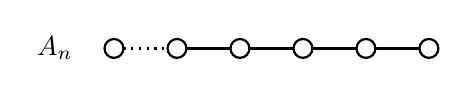
\begin{tikzpicture}[scale=.4]
    \draw (-1,0) node[anchor=east]  {$A_n$};
    \foreach \x in {0,...,5}
    \draw[xshift=\x cm,thick] (\x cm,0) circle (.3cm);
    \draw[dotted,thick] (0.3 cm,0) -- +(1.4 cm,0);
    \foreach \y in {1.15,...,4.15}
    \draw[xshift=\y cm,thick] (\y cm,0) -- +(1.4 cm,0);
  \end{tikzpicture}
\end{center}

There is a correspondence with each flag selecting one variety to a generator, though it is not a bijection.

The flag is composed by a vertex, an edge containing the vertex, a face containing the edge \ldots etc. If we focus on one variety, then the corresponding symmetry is the hyperplane $\rho $ that fixes the lower dimension varieties and keeps invariant the higher ones.

We will see it more clear in the next subsection.

\subsection{Classification of Platonic Solids}
There exist 5 platonic solids. We can think all the solids in the projective space to make easier computations.

\textbf{Tetrahedron $A_3$}

Vertices are the indicator vectors of $\binom{[4]}{1}$

We have a flag $\{V_1, V_2, V_3\}$, where $V_i$ are projective varieties that correspond to a vertex, edge and face respectively and for each  $V_i$ we have the induced hyperplane $\rho_i $ associated with the reflection $s_i$. If we compute the normal vectors of the planes:

 \[
\rho_1^\perp = \begin{pmatrix} 1\\-1\\0\\0 \end{pmatrix} , \quad
\rho_2^\perp = \begin{pmatrix} 0\\1\\-1\\0 \end{pmatrix} , \quad
\rho_3^\perp = \begin{pmatrix} 0\\0\\1\\-1 \end{pmatrix} \quad
\Rightarrow \quad
\angle \rho_1 \rho _2 = \frac{\pi}{3}, \quad
\angle \rho_1 \rho _3 = \frac{\pi}{2}, \quad
\angle \rho_2 \rho _3 = \frac{\pi}{3}
\] 
And then we deduce the diagram
% https://q.uiver.app/?q=WzAsMyxbMCwwLCJcXHRleHRjaXJjbGVkezF9Il0sWzEsMCwiXFx0ZXh0Y2lyY2xlZHsyfSJdLFsyLDAsIlxcdGV4dGNpcmNsZWR7M30iXSxbMCwxLCIiLDAseyJzdHlsZSI6eyJoZWFkIjp7Im5hbWUiOiJub25lIn19fV0sWzEsMiwiIiwwLHsic3R5bGUiOnsiaGVhZCI6eyJuYW1lIjoibm9uZSJ9fX1dXQ==
\begin{tikzcd}
	{\textcircled{1}} & {\textcircled{2}} & {\textcircled{3}}
	\arrow[no head, from=1-1, to=1-2]
	\arrow[no head, from=1-2, to=1-3]
\end{tikzcd}

\textbf{Cube $B_3$}

\textbf{Octahedron $B_3$}

Vertices are the indicator vectors of $\binom{[4]}{2}$

We have a flag $\{V_1, V_2, V_3\}$, where $V_i$ are projective varieties that correspond to a vertex, edge and face respectively and for each  $V_i$ we have the induced hyperplane $\rho_i $ associated with the reflection $s_i$. If we compute the normal vectors of the planes:

 \[
\rho_1^\perp = \begin{pmatrix} 1\\-1\\0\\0 \end{pmatrix} , \quad
\rho_2^\perp = \begin{pmatrix} 1\\0\\-1\\0 \end{pmatrix} , \quad
\rho_3^\perp = \begin{pmatrix} 1\\1\\-1\\-1 \end{pmatrix} \quad
\Rightarrow \quad
\angle \rho_1 \rho _2 = \frac{\pi}{3}, \quad
\angle \rho_1 \rho _3 = \frac{\pi}{2}, \quad
\angle \rho_2 \rho _3 = \frac{\pi}{4}
\] 
And then we deduce the diagram
\begin{tikzcd}
	{\textcircled{1}} & {\textcircled{2}} & {\textcircled{3}}
	\arrow[no head, from=1-1, to=1-2]
	\arrow["4", no head, from=1-2, to=1-3]
\end{tikzcd}

\textbf{Dodecahedron $H_3$}

\textbf{Icosahedron $H_3$}


\section{Description of Coxeter Groups}
\subsection{Group $A_n$}
\begin{tikzcd}
	\circ & \circ & \cdots & \circ & \circ
	\arrow[from=1-1, to=1-2]
	\arrow[from=1-2, to=1-3]
	\arrow[from=1-3, to=1-4]
	\arrow[from=1-4, to=1-5]
\end{tikzcd}

We can think type $A_n$ Coxeter Groups as groups generated by the reflections  $s_1, \ldots, s_{n-1}$ whose associated hyperplanes are defined by
\[
\rho_1 ^\perp = \begin{pmatrix} 1 \\ -1 \\ 0\\ \vdots \\ 0 \end{pmatrix} , \quad 
\rho_2 ^\perp = \begin{pmatrix} 0 \\ 1 \\ -1\\ \vdots \\ 0 \end{pmatrix} , \quad \ldots \quad
\rho_{n-1} ^\perp = \begin{pmatrix} 0 \\ \vdots \\ 0 \\ 1\\ -1 \end{pmatrix} , \quad 
\] 
It is easy to see that the angles between the hyperplanes are
\[
\angle \rho_i \rho_{i+1} = \frac{\pi}{3}, \quad 
\angle \rho_i \rho _{j} = \frac{\pi}{2}\ if\ i-j\neq \pm 1 \quad 
\] 
so that corresponds to the Dynkin diagram, and thus to the Coxeter group


\subsection{Group $B_n$}
\begin{tikzcd}
	\circ & \circ & \cdots & \circ & \circ
	\arrow["4", from=1-1, to=1-2]
	\arrow[from=1-2, to=1-3]
	\arrow[from=1-3, to=1-4]
	\arrow[from=1-4, to=1-5]
\end{tikzcd}

We can think type $B_n$ Coxeter groups as the group generated by the reflections  $\tau, s_1, \ldots, s_n$, whose associated hyperplanes are defined by
\[
\rho_\tau ^\perp = \begin{pmatrix} 1 \\ 0 \\ 0 \\  \vdots \\ 0 \end{pmatrix} , \quad 
\rho_1 ^\perp = \begin{pmatrix} 1 \\ 1 \\ 0\\ \vdots \\ 0 \end{pmatrix} , \quad 
\rho_2 ^\perp = \begin{pmatrix} 0 \\ 1 \\ 1\\ \vdots \\ 0 \end{pmatrix} , \quad \ldots \quad
\rho_n ^\perp = \begin{pmatrix} 0 \\ \vdots \\ 0 \\ 1\\ 1 \end{pmatrix} , \quad 
\] 

One can check that the angles between the hyperplanes are
\[
\angle \rho_\tau \rho _1 = \frac{\pi}{4}, \quad 
\angle \rho_\tau \rho _i = \frac{\pi}{2}\  if\ i>1, \quad 
\angle \rho_i \rho _{i+1} = \frac{\pi}{3}, \quad 
\angle \rho_i \rho _{j} = \frac{\pi}{2}\ if\ i-j\neq \pm 1 \quad 
\] 
so the construction correspond to the Dynkin diagram, and thus to the coxeter group.

\subsection{Group $D_n$}
\begin{tikzcd}
	\circ \\
	& \circ & \circ & \cdots & \circ & \circ \\
	\circ
	\arrow[from=2-2, to=2-3]
	\arrow[from=2-3, to=2-4]
	\arrow[from=2-4, to=2-5]
	\arrow[from=1-1, to=2-2]
	\arrow[from=3-1, to=2-2]
	\arrow[from=2-5, to=2-6]
\end{tikzcd}

We can think type $D_n$ Coxeter groups as the group generated by the reflections  $\tau_1, \tau_2, s_1, \ldots, s_n$, whose associated hyperplanes are defined by
\[
\rho_{\tau_1} ^\perp = \begin{pmatrix} 1 \\ 1 \\ 0 \\  \vdots \\ 0 \end{pmatrix} , \quad 
\rho_{\tau_2} ^\perp = \begin{pmatrix} -1 \\ 1 \\ 0\\ \vdots \\ 0 \end{pmatrix} , \quad 
\rho_1 ^\perp = \begin{pmatrix} 0 \\ 1 \\ 1\\ \vdots \\ 0 \end{pmatrix} , \quad \ldots \quad
\rho_n ^\perp = \begin{pmatrix} 0 \\ \vdots \\ 0 \\ 1\\ 1 \end{pmatrix} , \quad 
\] 

One can check that the angles between the hyperplanes are
\[
\angle \rho_{\tau_1} \rho _{\tau _2} = \frac{\pi}{2}, \quad
\angle \rho_{\tau_1} \rho _{1} = \frac{\pi}{3}, \quad
\angle \rho_{\tau_2} \rho _{1} = \frac{\pi}{3}, \quad
\angle \rho_i \rho _{i+1} = \frac{\pi}{3}, \quad 
\angle \rho_i \rho _{j} = \frac{\pi}{2}\ if\ i-j\neq \pm 1 \quad 
\] 
so the construction correspond to the Dynkin diagram, and thus to the coxeter group.


\section{Regular Subdivision and height functions}
Given a set of points $T$, we define a height function as  $h:T \to \mathbb{R}$.

The height function $h$ is said to be \textit{M-convex} if the regular subdivisions induced by $h$ are permutahedral.

A subset $S$ of points is a (lower) regular subdivision induced by $h$ if the convex hull of $S$ is described by the lower convex hull of the polytope $T\times h(T)$ 

\begin{definition}[3-Term Plücker Relations] Let $\omega $ be a height function.
For each $S\in \binom{[n]}{ d-2}$ and $i, j, k, l \not\in S$ the minimum
\[
\min (h(S_{ij}) + h(S_{kl}), h(S_{ik}) + h(S_{jl}), h(S_{il}) +  h(S_{jl}))
\] 
is attained at least twice.
\end{definition}

\begin{theorem}[] A height function induces a permutahedral regular division if the \textbf{3-Term Plücker Relations} (3TPR) holds.
\end{theorem}

\textbf{Proof.} 
We first translate what does it mean for the set of vertices $S_{ij}, S_{ik}, S_{il}, S_{jk}, S_{jl}, S_{kl}$ to be a regular subdivision induced by $h$. Trivially these 6 vertices form a subpermutahedron of  $P$. 

Now we have to see that the convex hull of the vertices is a lower convex hull of all the points. This means we can assign it a linear functional $\varphi = (\varphi _1, \ldots, \varphi_{n}, \varphi _{n+1}), \ \varphi _{n+1}>0$ that minimizes the set of 6 points over all the points. The consequence is that the functional evaluated in each of the 6 vertices should be equal. We abbreviate $h_{ij} := h(S_{ij})$

\begin{equation}
\varphi _{i_1} + \varphi _{i_2} + \varphi _{n+1}h_{i_{1}i_{2}} = \varphi _{i_3} + \varphi _{i_4} + \varphi _{n+1}h_{i_{3}i_{4}} \ \forall i_1, i_2 ,i_3, i_4 \in {i, j, k, l}
\end{equation}
\begin{equation}
\varphi _{i_1} - \varphi _{i_3} = \varphi _{n+1} (h_{i_3i_2}-h_{i_1i_2})
\end{equation}
\begin{equation}
  (\varphi _{i_2}-\varphi _{i_1})(h_{i_5i_7} - h_{i_6i_7}) = 
  (\varphi _{i_6}-\varphi _{i_5})(h_{i_1i_3} - h_{i_2i_3})
\end{equation}
Making now $i_1 = i_5$ and $i_2=i_6$ yields
\begin{equation}
h_{i_5i_7} - h_{i_{6}i_7} = h_{i_1i_3}-h_{i_2i_3} \quad or \quad \varphi _{i_2} = \varphi _{i_6}
\end{equation}

We observe that if all $\varphi _i$ are equal, then all the $h_{ij}$ should be equal by (1) and Plücker relations trivially hold.

Now suppose there is a






\end{document}





















